\section{Build Configuration [Rahat Rafiq]}\label{sec:build_config}

\begin{figure}
    \centering
    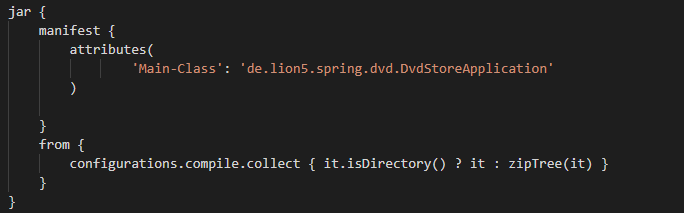
\includegraphics[width=14cm]{images/Rahat/fatJar.PNG}
    \caption{fatJar Generation}
    \label{fig:Generating_fatJar}
\end{figure}

Before configuring the CI pipeline it is necessary to change some build configuration of the application build tool Gradle. The first necessary step is to generate a jar file after each successful build of the application. Primarily Gradle has a default task in its build configuration that creates a boot jar of spring boot applications with every build. However, the boot jar does not contain application dependencies, thus it is not independently executable. So it is necessary to create a fatJar of the application with each build. A fat jar contains all the dependencies of the application thus it is independently executable. The efficient method to create a fatJar is to override the default task of the Gradle configuration file that creates the boot jar. \ref{fig:Generating_fatJar} Since the application will be deployed in a micro-service architecture, it is necessary to create a container image of the spring boot application. The fat jar will facilitate the creation of a docker containerized image of the application. Then it is also efficient to edit the application properties configuration of the application and update the data-source URL, credentials, and schema dialect to use a PostgreSQL database. It would provide developers the option of building, testing, and running the application in their local machine while utilizing a production-grade PostgreSQL database server for test cases. This added configuration removes the embedded database support from the spring boot application but the CI pipeline is also adjusted accordingly to accommodate this change.